\section{MPI parallelisation}
  \label{section:parallelisation:mpi}


\chapterDescription
  {
    180 minutes.
  }
  {
    A working simulation code and working MPI environment.
  }

In this section, we discuss how to parallelise a simulation code with message
passing.

\subsection{Preparation}

Peano relies on MPI with its SPMD paradigm, i.e.~all ranks run exactly the same
code.
Internally, it however creates a logical tree topology on all ranks. 
There is one rank that is the {\em global master}.
By convention, this is rank 0, i.e.~the very first rank launched by MPI.
All other ranks are {\em workers}.
Each rank besides the global master has one unique {\em master}.
Each worker can either be active, i.e.~participate in the computation, or it can
be idle.
At the begin of the simulation, all workers are idle and only the global master
is working (as it is working always).

The global master runs the actual Peano simulation code, holds the simulation
state and triggers the grid traversals.
Whenever it triggers a grid traversal, it tells all non-idle workers which
adapter is currently used.
It determines which algorithmic phase to run. 
Then, it starts to run through the grid. 
If parts of the grid are deployed to other ranks, they are informed to start a
traversal as well. 
The traversal kick-off propagates through the ranks along the master-worker
topology.
All of this is done automatically.
Most codes require the programmer to think only about the global master.

\paragraph{Re-translating the code.}
We expect that there is a command \texttt{mpicxx} available in your path.
This command often also is called \texttt{mpiCC}. Please ensure it calls the
right compiler backend. 
If you are unsure, check with argument \texttt{-V} and adopt the backend
manually if required. 

Change your compile command to \texttt{mpicxx} and add the two options
\begin{code}
  -DParallel -DMPICH_IGNORE_CXX_SEEK
\end{code}
to your compiler call.
While Peano is written in C++11, it relies only on C bindings of MPI.
Some MPI versions (mpich) have issues with this combination (give you tons of
warnings) unless you pass \texttt{MPICH\_IGNORE\_CXX\_SEEK}. 


\paragraph{Setting up the code.}

The auto-generated \texttt{main} calls Peano's operation \newline
\texttt{peano::initParallelEnvironment} which takes care of a proper MPI
initialisation. 
As soon as the initialisation has terminated without an error code, you may use
the predicate

\begin{code}
if (tarch::parallel::Node::getInstance().isGlobalMaster()) {
  ...
}
\end{code}

\noindent
to find out whether a particular piece of code runs on the global master. 
One of the first steps in many codes might be to perform some tests only on this
global master.
The counterpart \texttt{peano::shutdownParallelEnvironment()} typically is
invoked directly within \texttt{main} as well and is also called by the
autogenerated templates already.

As we follow SPMD, \texttt{main} has to create an instance of the runner and
invoke its \texttt{run} operation. 
The \texttt{run} then distinguishes between the global master and all the other
workers that blindfolded follow their masters. 
\begin{code}
  int result = 0;
  if (tarch::parallel::Node::getInstance().isGlobalMaster()) {
    result = runAsMaster( *repository );
  }
  #ifdef Parallel
  else {
    result = runAsWorker( *repository );
  }
  ...
\end{code}

\noindent
This code is generated and it is most of the time sufficient to focus on the
operation \texttt{runAsMaster}, i.e.~to focus on the serial code version. There
are however a few steps that have to be done on each individual worker
separately. 
You may implement this within the \texttt{main}.
However, we typically realise it within \texttt{run} just before or after the
operation splits up into the function for the global master and all other ranks.


{\bf Choose a load balancing request answering strategy on the global master}.
One for the first steps on the global master is to configure a
proper load balancing strategy. 
Peano realises a hybrid centralised-decentralised load balancing by default,
where load balancing decisions are, whenever possible, made centrally. 
Once load balancing decisions are made (along the lines `I would like more
ranks to help me with my work'), a central point is contacted that decides which
ranks are involved in the rebalancing.
This central point is called {\em node pool}.
Peano realises the whole node pool, but allows the user to plug into the
decisions which ranks are assigned to help which other ranks, e.g.
We have to configure the node pool on the global master only
\begin{code}
if (tarch::parallel::Node::getInstance().isGlobalMaster()) {
  tarch::parallel::NodePool::getInstance().setStrategy(
    new tarch::parallel::FCFSNodePoolStrategy()
  );
}
\end{code}

\noindent
where we select here one of the default strategies. 
It answers to any incoming load balancing request FCFS (while other strategies
might decide to bundle requests to get an overview who asks for resources first
before any rank assignment is performed) and hands out MPI ranks as long as
there are still idle workers available.

{\bf Restart the load balancing on all ranks}.
Once the node pool
is initialised, we have to restart it.
This has to be done on all ranks. 
On the global master, the operation really restarts the node pool.
On all other ranks, it establishes the connection to the central node pool
and informs the latter how many ranks are available.

\begin{code}
tarch::parallel::NodePool::getInstance().restart();
tarch::parallel::NodePool::getInstance().waitForAllNodesToBecomeIdle();
\end{code}

\begin{remark}
Many sophisticated load balancing schemes can deal with MPI ranks signing in and
out throughout the computation dynamically.
Peano per se can deal with dynamic rank allocation.  
However, the default FCFS strategy is not that elaborate. 
It requires that all ranks are well-known when it starts up and that they do not
change.
Therefore, it is mandatory to add the \texttt{waitForAllNodesToBecomeIdle()}
instruction here which ensures that all nodes register at the central node pool
and tell the central node pool strategy that they are idle and free for new
jobs. 
Though not mandatory, you might want to add this statement anyway at runtime to
ensure your whole system is up properly.
\end{remark}

\noindent
{\bf Configure the load balancing strategy on all ranks}.
In a next step, we configure the
actual load balancing.
Again, we rely on a default balancing that simply yields a static partitioning. 
This partitioning is established by a greedy grid decomposition while the grid
is built up.

\begin{code}
peano::parallel::loadbalancing::Oracle::getInstance().setOracle(
 new peano::parallel::loadbalancing::OracleForOnePhaseWithGreedyPartitioning(true)
);
\end{code}

\noindent
This trivial load balancing runs embarrassingly parallel on all ranks. 
The ranks do not communicate to come up with load balancing decisions.
In such a case, you could use different oracles on different ranks. 
In general, this is not a good idea and all ranks should run the same oracle.
 
\begin{remark}
Peano's MPI routines are written with the idea in mind that \texttt{#ifdef}s
pollute your code and basically introduce many different branches of your source
code that are more difficult to maintain than one single strand. The high level
MPI-related function calls thus all work in a serial code, too. If you
compile without \texttt{-DParallel}, they degenerate to nop (no operation), but
you always can be sure that everything compiles, is consistent and lots of
assertions are built in in non-release mode.
\end{remark}

\noindent 
{\bf Set buffer sizes on all ranks}.
MPI code tends to be very sensitive to proper buffer sizes.
In Peano, you have to ensure that all ranks work with the same buffer sizes
(otherwise the exchange of buffers will fail) and that you set them before you
actually exchange data. 
Please note that it is not recommended to change these buffer sizes throughout
any computation. 

\begin{code}
peano::parallel::SendReceiveBufferPool::getInstance().setBufferSize( bufferSize );
peano::parallel::JoinDataBufferPool::getInstance().setBufferSize( bufferSize );
\end{code}


\noindent
{\bf Configure deadlock time outs on all ranks (optional)}.
Peano's MPI communication routines all have some built-in deadlock detection. 
To enable it, you have to quantify what MPI waiting time is to be considered to
be a deadlock.
The deadlock identification is split into two phases.
A certain timeout interval first has to pass.
After it, a warning is launched. 
After a second timeout passes, the code is terminated.
It is reasonable to set these timeouts rather high if you run your code with
assertions or debug information.
To do all the checks and create debug data is time-consuming and thus might lead
into a deadlock identification though all nodes are busy creating the additional
information.
The other way round, many applications do not allow to run production runs with
assertions and debugs.
As deadlocks for small problems occur sooner than for large problems where
already MPI ill-balancing might yield long waiting times, they might realise the
waiting strategy exactly the other way round.

\begin{code}
  #if defined(Debug) || defined(Asserts)
  tarch::parallel::Node::getInstance().setDeadlockTimeOut(120*4);
  tarch::parallel::Node::getInstance().setTimeOutWarning(60*4);
  #else
  tarch::parallel::Node::getInstance().setDeadlockTimeOut(120);
  tarch::parallel::Node::getInstance().setTimeOutWarning(60);
  #endif
\end{code}

\noindent
{\bf Clean up all the ranks}.
It is finally good practice to make the node pool terminate just before
\texttt{run} has terminated.
You might also want to release all MPI datatypes Peano has created, as some
tools do complain if you don't so:

\begin{code}
tarch::parallel::NodePool::getInstance().terminate();
myprojectnamespace::repositories::RepositoryFactory::getInstance().
  shutdownAllParallelDatatypes();
\end{code}



\paragraph{Inside \texttt{runAsMaster}.}
Peano's \texttt{runAsMaster} for many application is MPI-agnostic.
Some applications run into problems if they use a grid setup in one sweep.
If Peano tries to decompose/load balance the initial grid, it might be forces to
postpone some \texttt{refine} calls on the grid. 
As a result, your grid initialisation should look similar to
\begin{code}
repository.switchToInitialGrid();
do {
  repository.iterate();
} while (!repository.getState().isGridBalanced());

logInfo(
  "runAsMaster()",
  "number of working ranks=" << 
  tarch::parallel::NodePool::getInstance().getNumberOfWorkingNodes() 
);
logInfo(
  "runAsMaster()",
  "number of idle ranks=" << tarch::parallel::NodePool::getInstance().getNumberOfIdleNodes()
);

\end{code}

\noindent
A serial code should continue to quit the \texttt{do} loop after one sweep. 
A parallel code might run through the grid several times.

\noindent
{\bf Two first, almost-parallel runs}.
Before you continue, I recommend to run your code with \texttt{mpirun} and only
one active process. 
Just ensure that your code continues to behave as the serial code does even
though MPI features are compiled into the sources.
Next, I recommmend you to run the code with two ranks and check whether
everything continues to work.

\begin{remark}
Peano by default implements a special policy for rank 0. Rank 0 is the global
master responsible for global load balancing decisions. Those decisions are
critical. 
Thus, rank 0 always deploys all work to other ranks and focuses exclusively on
load balancing and on running the overall algorithm control,
i.e.~\texttt{runAsMaster()}.
If you run the code with two MPI ranks, you should thus get similar runtime
results as with one rank.
\end{remark}
 
\begin{remark}
For fair and proper runtime comparisons, it might make sense to place the first
two MPI ranks on one CPU and make them share the resources.
Alternatively, you may want to reduce the number of actual ranks in your
measurements by one.
\end{remark}

\subsection{Exchanging the global state}

If Peano runs with MPI, the global master holds a repository which in turn holds
a solver \texttt{State}. 
This state is the globally valid state object. 
If the computational domain is split up, each \texttt{iterate} call within the
global master is subsequently distributed among all non-idle workers.
Together with this run information, the global master also distributes its state
object.
The state object is broadcasted to all ranks automatically (unless not switched
off explicitly as detailed below).

The \texttt{State}, the \texttt{Vertex} and the \texttt{Cell} objects are
modelled with DaStGen.
DaStGen also is responsible to configure proper MPI calls.
Every ``DaStGen'' object that is exchanged might be exchanged only partially:
indeed, DaStGen makes MPI exchange only those attributes that are explicitly
marked with \texttt{parallelise}.
The broadcast remark above thus has to be narrowed: 
Whenever you call \texttt{iterate}, the global master exchanges those properties
of its \texttt{State} instance that are marked to be exchanged. 
The object you receive in \texttt{beginIteration()} as state argument it exactly
this received object.

As soon as a worker terminates its traversal, it informs its master about this
termination.
This works recursively through the logical master-worker tree.
Again, Peano cares for the state transmission. 
However, any state object received from a worker is {\em not} merged into the
master. 
If you want to plug into the merge process, i.e.~if you want the global master
state to hold data from the other states in the end, you have to realise the
operation \texttt{mergeWithMaster} in any of your mappings.


\begin{center}
  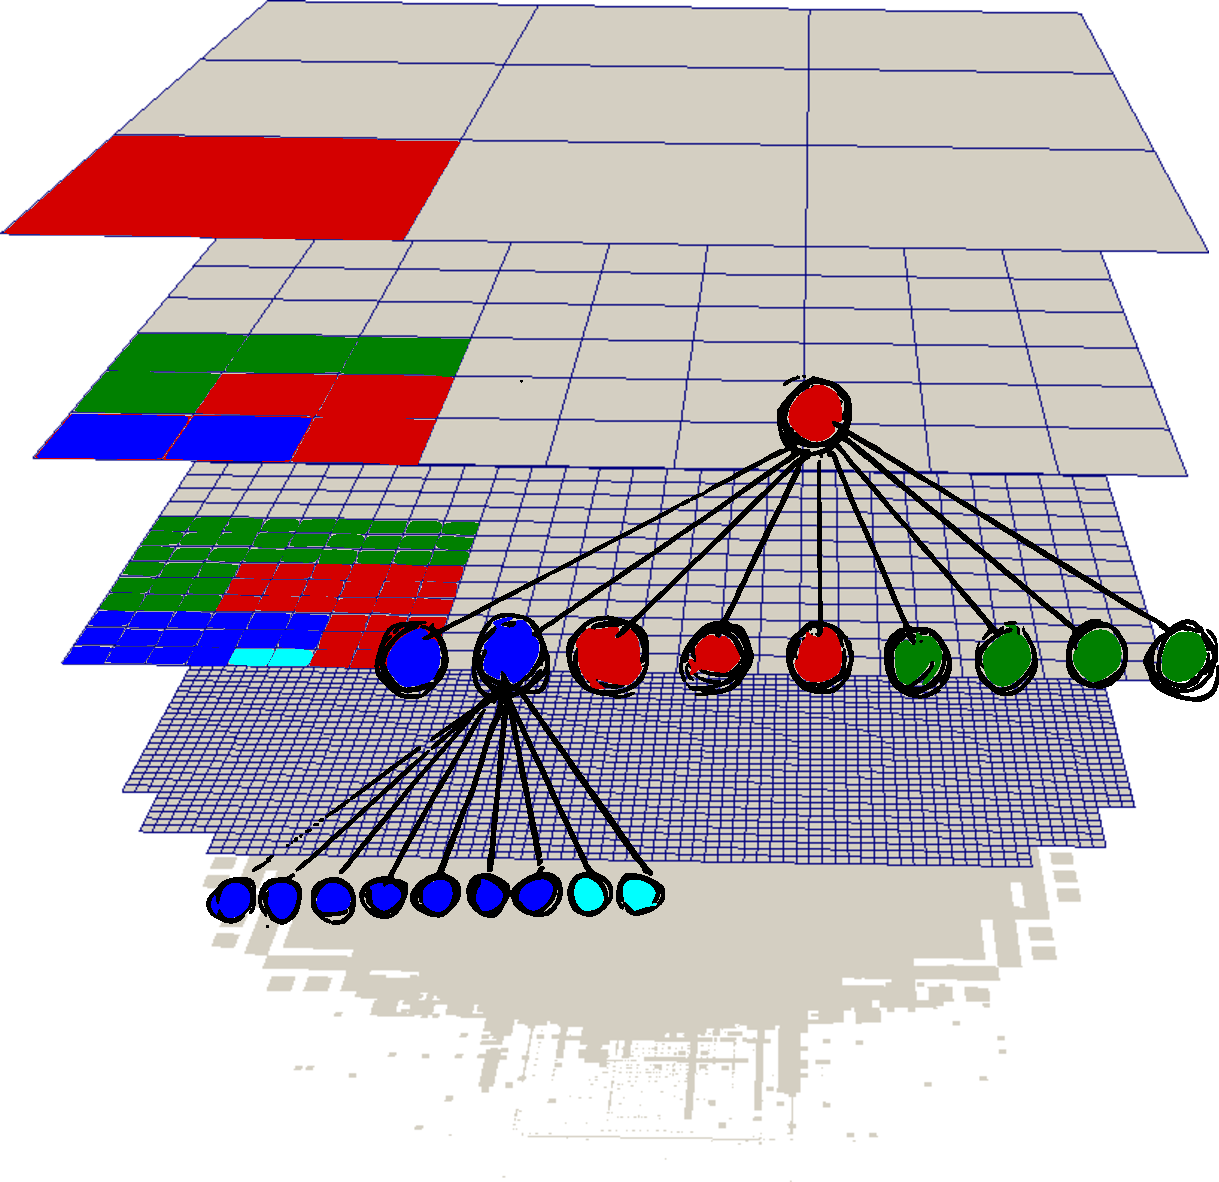
\includegraphics[width=0.5\textwidth]{52_mpi/spacetree-decomposition-top-down.pdf}
\end{center}

\noindent
The picture above details Peano's MPI concept:
The spacetree is top-down split up among the ranks. 
In the present fragment, red is the ``highest'' rank.
When it receives a \texttt{iterate} message from the global master, it also
receives a copy of the master's state as well as a copy of the coarsest cell
belonging to red and its adjacent vertices.
All these data is redundantly stored on the master.
The received state is automatically made the local state.
If you want to do something with the coarsest red cell or the four vertices
belonging to the coarsest level, you can realise 
\begin{code}
void mergeWithWorker(
  exahype::Cell&                               localCell, 
  const exahype::Cell&                         receivedMasterCell,
  const tarch::la::Vector<DIMENSIONS,double>&  cellCentre,
  const tarch::la::Vector<DIMENSIONS,double>&  cellSize,
  int                                          level
);

void mergeWithWorker(
  exahype::Vertex&                             localVertex,
  const exahype::Vertex&                       receivedMasterVertex,
  const tarch::la::Vector<DIMENSIONS,double>&  x,
  const tarch::la::Vector<DIMENSIONS,double>&  h,
  int                                          level
);
\end{code}

\noindent
in one of your mappings. Multigrid codes, e.g., might transfer residual through
the individual levels.

With all data received, the red node starts to traverse its own tree. 
It recognises that is in turn is the master to two other ranks (green and blue)
and forwards its received state to these guys---as well as the corresponding
cells and vertices on the coarsest common level that the master and its workers
hold redundantly.

Afterwards, red continues to run through its local tree. 
When it starts to ascend through its local tree, it waits for its two workers
(green and dark blue) to terminate and receives from them a state as well as
copies of their coarsest cell plus the adjacent vertices.
This time, the state is not merged into anything automatically. 
However, you can realise the corresponding merge operations to restrict a global
residual value for example.


\subsection{Exchanging boundary data}

Peano realises a non-overlapping domain decomposition on each individual
resolution level.
This means that no cells are held redundantly between two neighbouring ranks on
the same level (only the coarsest cell of any rank is held redundantly by its
master).
Boundary data exchange thus exclusively affects vertices. 
It is important to note that all vertices on all levels that are adjacent to
cells of different ranks are exchanged per iteration (unless not explicitly
switched off).

Again, the code does not literally exchange all data. 
It exchanges only those attributes of \texttt{Vertex} that are explicitly marked
with \texttt{parallelise} in the definition file.  

There are plug-in points where you can influence how data is exchanged along the
boundaries. The first plug-in point is the operation 

\begin{code}
void prepareSendToNeighbour(
  exahype::Vertex&                             vertex,
  int                                          toRank,
  const tarch::la::Vector<DIMENSIONS,double>&  x,
  const tarch::la::Vector<DIMENSIONS,double>&  h,
  int                                          level
);
\end{code}

\noindent
Whenever a rank finds out that it has just used a vertex for the very last time
throughout a traversal---this happens right after \texttt{touchVertexLastTime}
has been called---and that this vertex is adjacent to multiple ranks and thus
stored on multiple ranks, it calls \texttt{prepareSendToNeighbour} for this
vertex per communication partner \texttt{toRank}.
This operation gives every mapping the opportunity to plug into the send
mechanism.

Peano exchanges its data similar to the Jacobi scheme in linear algebra: 
at the end of an iteration, it sends away copies of vertices. 
Prior to the subsequent traversal, it receives this data and allows the user to
merge it into the local data structures.
For the latter, there is another plug in point:
\begin{code}
void mergeWithNeighbour(
  exahype::Vertex&                              vertex,
  const exahype::Vertex&                        neighbour,
  int                                           fromRank,
  const tarch::la::Vector<DIMENSIONS,double>&   x,
  const tarch::la::Vector<DIMENSIONS,double>&   h,
  int                                           level
);
\end{code}

\noindent
This operation hands you over the local vertex copy as well as the received data
from every other adjacent rank.
While Peano ensures that all grid refinement data, e.g., is kept consistently,
it is your job to ensure that all application-specific data is kept consistent.

A simple matrix-free Jacobi iteration on the vertices thus reads as follows:
\begin{enumerate}
  \item When a vertex is loaded for the very first time throughout a traversal,
  we set its residual to $0$. This happens in \texttt{touchVertexFirstTime()}.
  \item In \texttt{enterCell}, the local residual of this vertex is accumulated.
  \item As soon as we receive \texttt{touchVertexLastTime()} of a particular
  vertex, we know that the code has run through all adjacent cells before. The
  residual hence is complete and we can update the vertex solution according to
  the Jacobi update scheme.
\end{enumerate}

\noindent
This workflow transfers as follows to a distributed memory environment:
\begin{enumerate}
  \item When a vertex is loaded for the very first time throughout a traversal,
  we set its residual to $0$. This happens in \texttt{touchVertexFirstTime()}.
  \item In \texttt{enterCell}, the local residual of this vertex is accumulated.
  \item As soon as we receive \texttt{touchVertexLastTime()} of a particular
  vertex, we know that the code has run through all adjacent cells before {\em
  if the vertex is  a local one}. We can check this with the operation
  \texttt{isAdjacentToRemoteRank()}. The residual hence is complete and we can update the
  vertex solution according to the Jacobi update scheme.
  \item Of a vertex is adjacent to any other rank, we may not update its value.
  We know that this vertex is sent away at the end of the iteration through 
  \texttt{prepareSendToNeighbour}. We do not change any data of the vertex
  herein.
  \item Prior to the next \texttt{touchVertexFirstTime()} on any other rank, we
  know that this rank will receive our local copy of the vertex in
  \texttt{mergeWithNeighbour}. We thus make \texttt{mergeWithNeighbour} take any
  incoming vertex copy, take the residual from there and merge it into the local
  residual.
  \item If we run into \texttt{touchVertexFirstTime()} for a vertex with
  \texttt{isAdjacentToRemoteRank()}, we know that we didn't update its value yet
  because it had bee incomplete in the previous \texttt{touchVertexLastTime()}
  call. We however know that its residual is accumulated between domain
  boundaries now. We thus update and continue with the standard
  \texttt{touchVertexFirstTime()}.
\end{enumerate}



\subsection{Exchanging boundary data on the heap}

Different to the vertex boundaries, heap data is not automatically exchanged by
Peano's MPI. 
There are different variants how to manage heaps. 
The simplest one is to rely on the communication specification. 
Please ensure that one of your mappings defines a communication specification
that sets the third flag to \texttt{true}.
This instructs the Peano kernel that you want to use heaps for boundary data
exchange as well.
\begin{code}
peano::CommunicationSpecification  
myMapping::communicationSpecification() { 
  return peano::CommunicationSpecification( ...,...,true );
}
\end{code}

\noindent
Boundary data is also not transferred automatically. 
If you want to exchange data through a boundary vertex, you have to do so
explicitly in \texttt{prepareSendToNeighbour}.
Please note that Peano's heap has specialised operations for this:
\begin{code}
void myMapping::prepareSendToNeighbour(
  particles::pidt::Vertex&                      vertex,
  int                                           toRank,
  const tarch::la::Vector<DIMENSIONS,double>&   x,
  const tarch::la::Vector<DIMENSIONS,double>&   h,
  int                                           level
) {
  MyHeap::getInstance().sendData(
    index-of-heap-entry,
    toRank,
    x,
    level,
    peano::heap::NeighbourCommunication
  );
}
\end{code}

\noindent
The counterpart has to be realised in \texttt{mergeWithNeighbour}.
Peano takes care that all data is exchanged in the right order as efficiently as
possible.
You are however responsible to ensure that each heap send operation has a
corresponding receive on the other side for exactly the same vertex.
As the data exchange is distributed between two iterations, you might decide to
implement the receive in a different mapping.
However, you have to ensure that each send is mapped by exactly one receive on
the vertex counterpart.

\subsection{Running global steps on all ranks}

\subsection{Specifying the communication pattern}

\subsection{Doing something special on a worker}
